\chapter{Signalweiterleitung im biologischen Neuron}\label{ch:neuron}

Eingehende Signale empfängt eine Nervenzelle über seine \textbf{Dendriten}: Baumförmige Fortsätze, die um den Zellkörper - das \textbf{Soma} - herum gelagert sind\footnote{siehe Anhang~\ref{appendix:soma}}.
Sie fungieren \textit{postsynaptisch} und empfangen über \textbf{Rezeptoren} afferente\footnote{
  ``afferre`` (lat.): herbeibringen, melden, bringen
} Signale in Form von \textbf{Neurotransmittern}\footnote{ vgl.~\cite[61]{Eil19}.
 Oft stehen tausende Neuronen in Verbindung mit den Dendriten eines einzelnen Neurons (vgl.~\cite[42]{SD07}). Die Anzahl der Neuronen im menschlichen Gehirn beziffert sich auf mindestens $10^{11}$ (vgl.~\cite[175]{KSJ+13}).
} (siehe Abbildung~\ref{fig:neuron}).

\begin{figure}[h]
 \begin{center}
 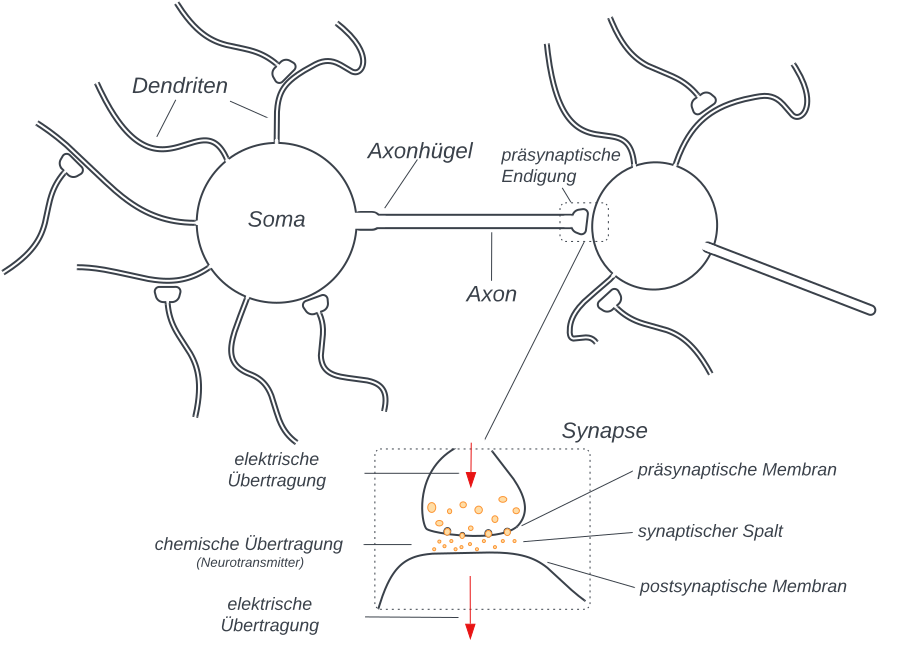
\includegraphics[
  width=16cm,
  keepaspectratio,
 ]{chapters/2. Das Neuron/images/nervenzelle}
 \caption{Aufbau einer Nervenzelle. (Quelle: in Anlehnung an~\cite[43, Tafel 2.1]{SD07})}
 \label{fig:neuron}
 \end{center}
 \small{
 Die Dendriten leiten afferente Signale zum Soma, dem Zellkörper. Das Axon leitet ein efferentes (``efferre``
  (lat.): hinaustragen, mitnehmen) Nervensignal über präsynaptische Endigungen (auch ``Axonterminale``) an (häufig weit entfernte) Effektoren wie Muskeln, Drüsen oder nachgeschaltete Neuronen weiter.}
\end{figure}

Dendriten leiten die Signale weiter an das Soma, in dem sich, durch die \textbf{Neuronenmembran}\footnote{
 Membrandicke ca. 5 nm (vgl.~\cite[66]{FE19})
} von der Umgebung getrennt, \textbf{Zytosol} befindet: Eine salzige, wässrige Flüssigkeit mit einem hohen Anteil von Kalium\footnote{vgl.~\cite[29]{BCP18}. Siehe hierzu auch ``Ionenkonzentrationen`` in Tabelle~\ref{tab:ionenkonzentration}.
}.

Ob das Neuron Signale weiterleitet, entscheidet sich in der Nähe des \textbf{Axonhügels}\footnote{
 ca. 20 - 50 µm vom Soma entfernt~\cite[77]{Jon19}
}: Hier entspringt das \textbf{Axon}\footnote{
 ``axon`` (lat.): Achse; Axone können sich im menschlichen Körper über Entfernungen von bis zu über 1m ausstrecken~\cite[28]{BCP18}
}, das in einer ``salzigen extrazellulären Flüssigkeit mit hoher Leitfähigkeit`` liegt~\cite[61]{BCP18}\footnote{
 \textit{Bear et al.} führen das Axon metaphorisch mit einer Telefonleitung zusammen (siehe~\cite[43]{BCP18}). Aufgrund der signalempfangenden Eigenschaften und der dünnen Spitzen der Dendriten werden diese auch mit Antennen verglichen (siehe~\cite[28]{BCP18})
}. Reicht die Integration der durch die postsynaptischen Endigungen eingehenden Signale aus, kann eine Depolarisation\footnote{
  \textit{Depolarisation} bezeichnet die Verringerung des Membranpotenzials von einem negativen Wert auf einen weniger negativen oder gar einen positiven Wert (vgl. ~\cite[95 f.]{SBB+13})
} der Membran an dieser Stelle\footnote{vgl.~\cite[61]{Eil19}} erfolgen. Wird ein gewisser \textbf{Schwellenwert} übertroffen, wird ein \textbf{Aktionspotenzial} ausgelöst (vgl.~\cite[142 f.]{BCP18}), was in den präsynaptischen Endigungen die \textbf{Exozytose}\footnote{
  bezeichnet den Stofftransport aus der Zelle heraus.
} auslöst.


\section{Ionenkonzentrationen und Membranspannungen}\label{sec-ionenkonzentrationen}

Ein Neuron weist \textit{in Ruhe}\footnote{
 vgl. \textbf{Mempranpotenzial}: ``die Spannung an der Nervenzellmembran zu einem beliebigen Zeitpunkt``~\cite[70]{BCP18}; \textbf{Ruhepotenzial}: ``the electrical potential across the membrane in the absence of signaling``~\cite[126]{KSJ+13}
} eine ungleiche Ionenverteilung zwischen der durch die Zellmembran getrennten intrazellulären Flüssigkeit (das Zytosol, im folgenden auch IZF) und der extrazellulären Flüssigkeit (im folgenden EZF) auf.
In der IZF befinden sich mehr positiv geladene Natrium-Ionen ($Na^+$), und in der EZF mehr positiv geladene Kalium- und Calcium-Ionen ($K^+$ und $Ca^{2+}$) sowie mehr negativ geladene Chlorid-Ionen ($Cl^-$).

{\renewcommand{\arraystretch}{1.5}%
\begin{table} %[hbtp]
 \centering
 \begin{tabular}{l | c | c | c }
  \textbf{Ion} & \textbf{Konzentration EZF (mmol/l)} & \textbf{Konzentration IZF (mmol/l)} & \textbf{Verhältnis} \\
  \hline
  $K^+$      & 5 & 100 & 1 : 20 \\
  $Na^+$     & 150 & 15 & 10:1 \\
  $Ca^{2+}$  & 2 & 0,0002 & 10000 : 1 \\
  $Cl^-$     & 150 & 13 & 11,5 : 1 \\
 \end{tabular}
 \caption{Ionenkonzentration eines Neurons in Ruhe (Quelle: ~\cite[75, Abb. 3.15]{BCP18})}
 \label{tab:ionenkonzentration}
\end{table}


Das \textbf{Membranpotenzial} des Neurons wird durch die Verteilung der Ionen in der IZF und EZF bestimmt: In der Membran befinden sich \textbf{Ionenkanäle}, von denen viele \textbf{selektiv permeabel}\footnote{
 von ``\textit{permeare}`` (lat.) durchwandern.
 Ein selektiv permeabler Kanal ist nur für bestimmte Ionen durchlässig (\textit{ionenselektiv}). Kaliumkanäle sind durchlässig für $K^+$-Ionen, Natriumkanäle durchlässig für $Na^+$-Ionen usw. (vgl.~\cite[66]{BCP18}).
 Die Kanäle können über Änderungen in der Umgebung des Neurons geöffnet oder geschlossen werden, was auch als \textbf{Gating} bezeichnet wird (vgl.~\cite[108]{KSJ+13})
} sind.
Daneben existieren \textbf{Ionenpumpen} wie die $Ca^{2+}$- und $Na^+$-$K^+$-ATPasen. Sie sorgen dafür, dass im Neuron laufend $Ca^{2+}$ und $Na^+$ aus der Zelle und $K^+$ in die Zelle befördert wird (vgl.~\cite[44]{SD07}). Zusammen mit den selektiv permeablen Ionenkanälen entstehen so die Ionenkonzentrationen in Tabelle~\ref{tab:ionenkonzentration}.\\


Wenn kein \textbf{postsynaptisches Potenzial} (PSP) wirkt und das Neuron selber keinen Impuls abgibt, liegt das Ruhepotenzial $V_r$ der Zelle zwischen $-70 mV$ und $-90 mV$\footnote{
   vgl.~\cite[47, Tafel 2.3 (A.1)]{SD07}. \textit{Bear et al.} geben $-65 mV$ an ($1 mV = 0,001 V$), also wird von einer 40-mal höheren Ionenpermeabilität für $K^+$ gegenüber $Na^+$ ausgegangen (vgl.~\cite[74, Exkurs 3.2]{BCP18} sowie~\cite[70]{BCP18})
}: Das Zytosol weist entlang der Membranoberfläche in der IZF eine negative Ladung auf\footnote{
 vgl.~\cite[61]{BCP18}. Das Membranpotenzial $V_m$ ergibt sich als die Differenz der Spannungen $V_{IZF}$ und $V_{EZF}$, wobei $V_{IZF}$ die Spannung in der IZF und $V_{EZF}$ die Spannung in der EZF ist. $V_r$ ist dann gleich zu $V_{IZF}$: Wenn die Zelle in Ruhe ist, wird die Spannung in der EZF als $0$ festgelegt (vgl.~\cite[127]{KSJ+13}).
}.
Diese \textbf{Membranspannung} $V_m$ wird durch eine ungleiche Ionenverteilung bewirkt, verursacht durch die Ladung der Teilchen in der IZF und EZF in Membrannähe\footnote{vgl.~\cite[66]{FE19}. \textit{Bear et al.} stellen fest:
 ``Die negativen Ladungen im Inneren des Neurons und die positiven Ladungen außerhalb des Neurons ziehen sich in Richtung Zellmembran gegenseitig an, {[...]} Dementsprechend ist die negative Nettoladung im Inneren der Zelle nicht gleichmäßig im Cytosol verteilt, sondern an der Innenseite der Membran lokalisiert.``~\cite[72, Punkt 2]{BCP18}
} (siehe Abbildung~\ref{fig:ionenverteilung}).\\


\begin{figure}[htpb]
 \begin{center}
 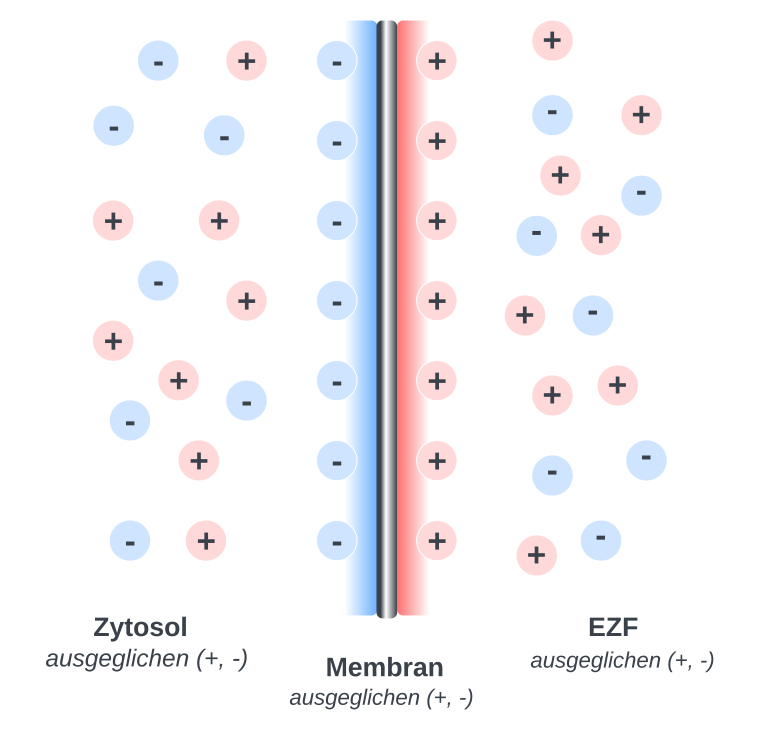
\includegraphics[
  width=8cm,
  keepaspectratio,
 ]{chapters/2. Das Neuron/images/ionenverteilung}
 \caption{Ionenverteilung im Zytosol und der EZF. (Quelle: in Anlehnung an~\cite[72, Abb. 3.13]{BCP18})}
 \label{fig:ionenverteilung}
 \end{center}
 \small{
  Aufgrund der elektrostatischen Anziehungskraft ziehen sich Anionen (neg. geladen) und Kationen (pos. geladen) in der Nähe der Membran gegenseitig an, es kommt zu einer negativen Spannung in Membrannähe (zwischen $-70 mV$ und $-90 mV$ in Ruhe). Dadurch ist die negative Ladung nicht gleichmässig im Zytosol verteilt. \textit{Bear et al.} weisen darauf hin, dass trotzdem der größte Teil des Zytosols und der EZF elektrisch neutral ist (vgl.~\cite[72, Abb. 3.13]{BCP18})}
 }
\end{figure}

In Ruhe ist die Leitfähigkeit der Membran für $Na^+$ gering, für $K^+$ hingegen hoch (vgl.~\cite[44]{SD07}).
$K^+$-Ionen folgen ihrem \textbf{Konzentrationsgradienten} und gelangen über die Ionenkanäle in die EZF, bis die \textbf{Potenzialdifferenz} entlang der Neuronenmembran ausströmende $K^+$-Ionen zurückhält: Wenn diese Differenz den Konzentrationsgradienten für $K^+$ kompensiert, ist das \textbf{Gleichgewichtspotenzial} erreicht, und es findet keine Nettoionenbewegung statt\footnote{
 vgl. ~\cite[72]{BCP18}. \textit{Kandel et al.} schreiben hierzu:
 ``the equilibrium potential of any ion that is present on both sides of a membrane permeable to that ion``~\cite[130]{KSJ+13}
}.

Es gilt, dass sich das Membranpotenzial dem Gleichgewichtspotenzial desjenigen Ions annähert, für das die Membran besonders permeabel ist (vgl. ~\cite[145 f.]{KSJ+13}): Bestimmen lässt sich das Gleichgewichtspotenzial für individuelle Ionen mit der Nernst-Gleichung\footnote{
 vgl.~\cite[67]{FE19}.
} (s. Gleichung~\ref{eq:gl-nernst} sowie Tabelle~\ref{tab:nernstkonstanten}):\\

\textit{Bear et al.} definieren\footnote{siehe ~\cite[74, Exkurs 3.2]{BCP18}}:
\begin{equation}
E_{Ion} = 2,303  \times \begin{matrix} RT \\ \hline zF \end{matrix} \times log_{10} \times \begin{matrix} [Ion]_{EZF} \\ \hline [Ion]_{IZF} \end{matrix}
\label{eq:gl-nernst}
\end{equation}



  {\renewcommand{\arraystretch}{1.5}%
\begin{table} %[hbtp]
\begin{center}
 \begin{tabular}{l |l }
  \textbf{Variable / Konstante} & \textbf{Bedeutung}  \\
  \hline
  $E_{ion}$            & Gleichgewichtspotenzial für das jeweilige Ion \\
  $R$                  & Gaskonstante \\
  $T$                  & absolute Temperatur \\
  $z$                  & Ladungszahl des Ions \\
  $F$                  & Faraday-Konstante \\
  $[Ion]_{EZF}$        & Ionenkonzentration \textbf{ausserhalb} der Zelle \\
  $[Ion]_{IZF}$        & Ionenkonzentration \textbf{innerhalb} der Zelle \\
 \end{tabular}
 \caption{Nomenklatur Nernst-Gleichung}
 \label{tab:nernstkonstanten}
\end{center}
 \small{
$E$: \textit{Equilibrium} (``Gleichgewicht``); \textit{Faraday-Konstante}: elektrische Ladung eines Mols einfach geladener Ionen; 1 Mol = $6.02214076e10^{23}$ Teilchen

}

\end{table}

\noindent
Für eine Körpertemperatur von 37° lässt sich die Nernst-Gleichung für das Gleichgewichtspotenzial $E_K$ wie folgt vereinfachen:

\begin{equation}
 E_{K} = 61,54 mV  \times log_{10} \begin{matrix} [K^+]_{EZF} \\ \hline [K^+]_{IZF} \end{matrix}
 \label{eq:gl-nernst-reduced-start}
\end{equation}

\noindent
Mit den Werten aus Tabelle~\ref{tab:ionenkonzentration}  ergibt sich somit


\begin{equation}
E_{K} = 61,54 mV  \times log_{10} \begin{matrix} 1 \\ \hline 20 \end{matrix} \approx -80 mV
\label{eq:gl-nernst-reduced-end}
\end{equation}

\noindent

Zur Bestimmung von $V_m$ einer für mehrere Ionen permeablen Membran kann die \textbf{Goldman-Gleichung}\footnote{
 siehe Anhang~\ref{appendix:goldman}
} verwendet werden:

\begin{equation}
V_{r} = \begin{matrix} RT \\ \hline F \end{matrix}  \times ln \begin{matrix}
  P_{Na} \space  \times \space [Na^+]_{EZF} \space + \space P_{K} \space  \times \space [K^+]_{EZF} \space + \space P_{Cl} \space  \times \space [Cl^-]_{IZF}  \\ \hline
  P_{Na} \space  \times [Na^+]_{IZF} \space + \space P_{K} \space  \times \space [K^+]_{IZF} \space + \space P_{Cl} \space  \times \space [Cl^-]_{EZF}
\end{matrix}
\label{eq:gl-goldman}
\end{equation}

Eine weitere wichtige Eigenschaft der Membran ist die \textit{elektrische Leitfähigkeit} $g_{Ion}$; für sie gilt, dass sie proportional zu der Anzahl der offenen Ionenkanäle $N_{Ion}$ ist (vgl.~\cite[93]{BCP18}).

\section{Das Aktionspotenzial}\label{sec:aktionspotenzial}

In Ruhe ist die Ladung in Membrannähe in der IZF negativ, in der EZF positiv.
Durch eine schnelle Umkehrung dieser Verhältnisse ist eine Nervenzelle dazu in der Lage, ein Signal auszulösen (vgl.~\cite[86]{BCP18}).
Hierzu bedarf es eines \textbf{Aktionspotenzials}, das durch Ionenbewegungen entsteht. Die Ionenbewegungen selber sind auf die Änderung des Membranpotenzials zurückzuführen, wodurch ein Öffnen oder Schliessen von ionenspezifischen Kanälen verursacht wird (vgl.~\cite[96]{BCP18}).

 \textit{Kandel et al.} führen 4 wichtige Eigenschaften des Aktionspotenzials auf (vgl.~\cite[148 f.]{KSJ+13}):
\begin{enumerate}
 \item Es gibt einen \textbf{Schwellenwert} für die Auslösung des Potenzials.
 \item Das Aktionspotenzial ist ein \textbf{Alles-oder-Nichts} Ereignis.
 \item Das Aktionspotenzial wird ohne Verlust weitergeleitet.
 \item Nach dem Auslösen des Aktionspotenzial kommt es zu einer \textbf{Refraktärzeit}, in der zunächst kein weiteres Aktionspotenzial ausgelöst werden kann (\textbf{absolute Refraktärzeit}). Bevor $V_r$ wieder erreicht ist, wird für eine kurze Dauer ein stärkeres Signal benötigt, um das Aktionspotenzial erneut auszulösen (\textbf{relative Refraktärzeit})\footnote{
   beide Zeitabschnitte sind Teil der \textbf{Nachhyperpolarisation}, dargestellt in in Abbildung~\ref{fig:aktionspotenzial}.  Bei der ``Hyperpolarisation`` ändert sich das Membranpotenzial auf negative Werte in Richtung $V_r$ und darunter und wird in diesem Kontext als Hemmung verstanden.
}
\end{enumerate}


\subsection{Auslösung eines Aktionspotenzials}

\begin{figure}[h]
 \centering
 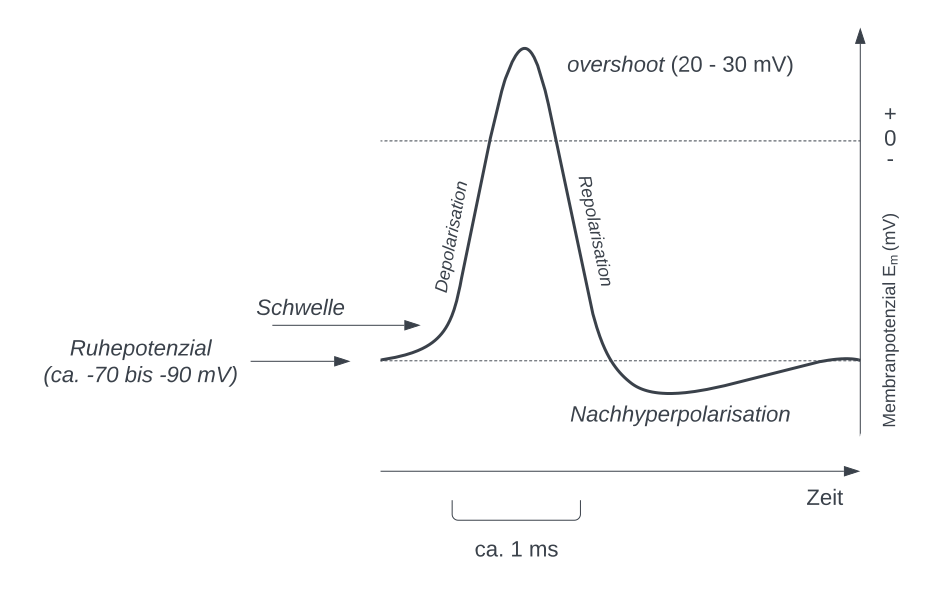
\includegraphics[
  width=12cm,
  keepaspectratio,
 ]{chapters/2. Das Neuron/images/aktionspotenzial}
 \caption{Aktionspotenzial. (Quelle: in Anlehnung an~\cite[47, Tafel 2.3]{SD07})}
 \label{fig:aktionspotenzial}
 \end{figure}


Die \textbf{Initiationszone}~\cite[111]{BCP18} des Aktionspotenzials ist der Axonhügel. Hier findet sich eine besonders dichte Anhäufung von spannungsabhängigen $Na^+$-Kanälen\footnote{
 pro Quadratmikrometer (µm²) kann eine Membran viele tausend Natriumkanäle enthalten~\cite[99]{BCP18}
}, deren Aktivierungskurve um ca. $10 mV$ zu den negativen Membranpotenzialen verschoben ist, was die Initiierung des Signals begünstigt (vgl. ~\cite[77]{Jon19}).

Damit ein Aktionspotenzial ausgelöst werden kann, muss die Membran nahe der Initiationszone über ihren \textbf{Schwellenwert} \footnote{
 ``das kritische Niveau der Depolarisation, das überschritten werden muss, um ein Aktionspotenzial auszulösen``~\cite[88]{BCP18} oder auch ``Erregungsschwelle``~\cite[69]{FE19}
} $V_t$ ( > $V_r$ ) depolarisiert werden (vgl.~\cite[111]{BCP18}).


 Als Schwellenwert wird das Membranpotenzial bezeichnet, bei dem die Permeabilität für $Na^+$ größer als für $K^+$ ist (vgl.~\cite[103]{BCP18})\footnote{$V_r$ ist in Ruhe nahe an $E_K$.}; $V_t$ liegt bei ca. $- 50mV$, unabhängig vom Typ des Neurons (vgl.~\cite[75]{Jon19}).
 Damit sich $V_r$ an $V_t$ nähert, bedarf es einer Erregung der Zelle durch postsynaptische Potenziale (vgl. ~\cite[69]{FE19}) oder ``eine aus der Umgebung weitergeleitete (elektrotonische) Erregung``~\cite[46]{SD07}.

Die Stärke der Erregung der Zelle ist entscheidend für das Auslösen eines Aktionspotenzials. Es muss mehr $Na^+$ in die Zelle einströmen, als $K^+$ aus der Zelle ausströmen kann (vgl.~\cite[69]{FE19}).
Versuche zeigen, dass die Potenzialänderung der Membran in einem Bereich von $-80 mV$ zu $-65 mV$ in dieser Hinsicht kaum Änderung bewirkt (vgl.~\cite[99]{BCP18}). $g_{Na}$ erhöht sich, aber wenn $V_r$ nicht erreicht wird, bleibt es bei dieser ``lokalen Antwort``~\cite[46]{SD07}. Erst eine Depolarisation der Membran hin über diesen Wert\footnote{
 ab -60 mV gehen die Natrium-Kanäle in den Offen-Zustand über (vgl.~\cite[69]{FE19}).
} kann die \textbf{Initiationsphase}\footnote{siehe ~\cite[68]{FE19}} des Aktionspotenzials einleiten: Es öffnen sich mehr Natrium-Kanäle, und durch die negative Ladung der Membran-Innenseite gibt es eine starke elektrochemische Triebkraft für $Na^+$-Ionen (vgl.~\cite[103]{BCP18}). Die Triebkraft ist zu diesem Zeitpunkt die Differenz des Membranpotenzials $V_m$ und $E_{Na}$. Bei $-60 mV$ beträgt die Triebkraft\footnote{
 vgl.~\cite[39]{Fak19}
}:

 \begin{equation}
  V_m - E_{Na} = -60 mV - 61,54 mV = -121,54 mV
  \label{eq:gl-triebkraft}
 \end{equation}


Da sich durch zunehmende Öffnung der Natrium-Kanäle $g_{Na}$ erhöht, strömen aufgrund der hohen Triebkraft für $Na^+$ mehr $Na^+$-Ionen in das Zellinnere. Es kommt zu einem \textbf{Rückkopplungseffekt} , denn die zunehmend weniger negative Membranspannung öffnet weitere Natrium-Kanäle, die Leitfähigkeit der Membran wird weiter erhöht und es kommt zu einem exponentiellen Anstieg der $Na^+$-Konzentration in der IZF. Der ``explosionsartige`` Natriumeinstrom bewirkt die Depolarisation der Membranspannung und das Aktionspotenzial wird ausgelöst (vgl.~\cite[69]{FE19})\footnote{
siehe hierzu auch Anhang~\ref{appendix:aktionspotenzial}
}.

Die Stärke des Signals selber ist unabhängig von dem Wert, der zu der überschwelligen Reizung des Neurons geführt hat: Amplitude und Zeitverlauf des Signals im Axon hängen nicht von Intensität und Dauer des Reizes ab (vgl.~\cite[75]{Jon19}). Entweder kommt es zu einem Aktionspotenzial, oder es bleibt bei einer lokalen Antwort. Aus diesem Grund funktionieren Aktionspotenziale nach dem \textbf{Alles-oder-Nichts-Prinzip}\footnote{vgl.~\cite[89]{BCP18}. Außerdem:
 ``Im Computerzeitalter bezeichnet man das axonale Aktionspotenzial auch als 'digitales' Signal.``~\cite[75]{Jon19}. \tetxit{Frank} bietet eine Übersicht über die Erforschung des Alles-oder-Nichts-Prinzip in~\cite{Fra94}. Dort wird \textit{Lucas} erwähnt, der 1905 in~\cite{Luc05} die Kontraktionen von Muskelfasern unter diesem Gesichtspunkt untersucht hat (vgl.~\cite[210]{Fra94})
}:

\blockquote[{\cite[157]{KSJ+13}}]{
 ``A fraction of a millivolt can be the difference between a subthreshold stimulus and a stimulus that generates a full-sized action potential.``
}

\subsection{Signalweiterleitung über das Axon}

Kurz nach der Aktionspotenzialbildung befinden sich daran beteiligte Membrane in der Refraktärphase, ihre $Na^+$-Kanäle sind inaktiviert. 
Somit pflanzt sich das Aktionspotenzial nur in eine Richtung fort\footnote{\textit{orthodrome} Fortleitung.
  \textit{Bear et al.} verweisen auf \textit{antidrome} Fortleitung, die in Experimenten ausgelöst werden kann~\cite[106]{BCP18}
} (vgl.~\cite[106]{BCP18}).
Die Fortleitung geschieht in Richtung der Axonterminal, wo sich die präsynaptischen Endigungen befinden und das elektrische Signal in chemische Signale umgewandelt werden (siehe Abbildung~\ref{fig:neuron}).


\section{Synaptische Übertragung und Integration}


\subsection{Synaptische Übertragung}\label{sec:synaptischeuebertragung}
Neben elektrischen Synapsen, bei denen der Signalaustausch durch einen direkten Stromfluss über sogenannte \textit{gap junctions} und deren ionenleitfähige Verbindungen\footnote{
 ``\textit{Konnexone}``; vgl.~\cite[50]{SD07}
} passiert (vgl.~\cite[119]{BCP18}), erfolgt die Signalweiterleitung im Gehirn überwiegend auf chemische Weise (vgl.~\cite[121 ff.]{BCP18}).

Chemische Synapsen sind nicht direkt miteinander verbunden. 
Zwischen ihnen existiert ein Spalt, der ca. $20$ - $40 nM$ breit ist (vgl.~\cite[184]{KSJ+13}), und in der sich eine Matrix aus extrazellulären Proteinen befindet\footnote{
 die \textit{extrazelluläre Matrix}. Hierbei handelt sich um den Gewebeanteil im \textit{Interzellularraum}, also der Raum ausserhalb der Zellen: ``The extracellular matrix {[...]} surrounds all connective tissue cells providing mechanical support and physical strength to tissues, organs and the organism as a whole``~\cite[3]{AHH+98}
}, die den Synapsenspalt überbrückt (vgl. ~\cite[122]{BCP18}).
Die Übertragung von Signalen erfolgt über Exozytose: Botenstoffe (\textit{Neurotransmittern}) diffundieren aus den präsynaptischen Endigungen in diesen Spalt (vgl.~\cite[122]{BCP18}). Rezeptoren an den postsynaptischen Endigungen wandeln die Botenstoffe in hemmende oder erregende Signale um, die dann von der postsynaptischen Zelle nach dem Alles-oder-Nichts-Prinzip integriert werden\footnote{siehe hierzu auch Anhang~\ref{appendix:neurotransmitter}}.\\

Die durch das Aktionspotenzial ausgelöste Depolarisation der Membran an den Axonterminalen bewirkt eine Öffnung spannungsgeladener Calcium-Kanäle (vgl.~\cite[184]{KSJ+13}).
Durch die ungleiche $Ca^{2+}$-Ionenkonzentration zwischen der EZF und IZF (10.000 : 1, siehe Tabelle~\ref{tab:ionenkonzentration}) entsteht eine hohe Triebkraft für $Ca^{2+}$: Nach Gleichung~\ref{eq:gl-nernst} ergibt sich für das Gleichgewichtspotenzial für $Ca^2+$

\begin{equation}
 E_{Ca^{2+}} = 123,08 mV
 \label{eq:gl-eqca2}
\end{equation}


und bei einem Membranpotenzial von $V_m \sim 20 mV$ durch Depolarisation liegt die Triebkraft für $Ca^{2+}$ bei $\sim -100 mV$:

\begin{equation}
 V_m - E_{Ca^{2+}} = 20 mV - 123,08 mV = -103,08 mV
 \label{eq:gl-triebkraftca2}
\end{equation}


Die Calcium-Ionen strömen in das Innere der Zelle und lösen die Exozytose von \textbf{synaptischen Vesikeln}\footnote{
 ``\textit{vesicula}`` (lat.): ``Bläschen``
} aus, kleine, mit einer Membran von der IZF getrennte Strukturen von etwa $50 nm$ Durchmesser, die mit Neurotransmittern gefüllt sind (vgl.~\cite[1000]{BCP18}).
Im \textit{synaptischen Endknöpfchen} befinden sich 100--200 von diesen Bläschen, die jeweils tausende Moleküle eines Neurotransmitters beinhalten (vgl.~\cite[184]{KSJ+13}).

Der Calciumeinstrom in die präsynaptische Endigung löst die Verschmelzung dieser Bläschen mit der Zellmembran des Endknöpfchens an der sogenannten \textbf{aktiven Zone}\footnote{
 \textit{Bear et al.} beschreiben das Aussehen der aktiven Zone als ``ein Feld winziger Pyramiden``~\cite[123]{BCP18}; \textit{Rohkamm und Kerner} erklären die direkte Einwirkung (ionotrop) und indirekte Einwirkung (metabotrop) der Neurotransmitter (siehe. ~\cite[134]{RK18})
} aus: Ein spezialisierter Abschnitt der Membran, der direkt gegenüber der \textbf{postsynaptischen Dichte} liegt\footnote{
 damit ist der Abschnitt der postsynaptischen Endigung gemeint, in der sich die Rezeptoren befinden (vgl.~\cite[96]{HS19a})
}\footnote{
Kurz nach Beginn der Transmitterübertragung über den synaptischen Spalt findet die \textbf{Endozytose} statt, ein Recyclingprozess, in dem die individuellen Vesikelmembranen wiederhergestellt und mit Neurotransmitter erneut aufgefüllt werden (vgl.~\cite[133]{BCP18}).
}



\subsection{Synaptische Integration}

Die Neurotransmitter eines einzelnen Vesikels lösen einen minimalen exzitatorischen oder inhibitorischen postsynaptischen Strom aus (\textbf{mEPSC} bzw. \textbf{mIPSC}, \textit{miniature excitatory / inhibitory postsynaptic current})\footnote{
EPSCs und IPSCs setzen sich aus einzelnen dieser mEPSC bzw. mIPSC zusammen und bilden die kleinste Einheit der postsynaptischen Ströme, weshalb man sie als \textit{Quanten} bezeichnet~\cite[98]{HS19a}.
Da EPSPs ein Vielfaches des Quantums sind, ``das die Menge an Transmitter in einem einzigen Vesikel und die Anzahl der postsynaptischen Rezeptoren an der Synapse widerspiegelt``, nennt man sie ``gequantelt``~\cite[142]{BCP18}. Mit Hilfe der \textbf{Quantelungsanalyse} lässt sich die Anzahl der an einer synaptischen Übertragung beteiligten Vesikel bestimmen (vgl. \cite[142]{BCP18}).
}.

Wesentlich für die Entstehung eines neuen Aktionspotenzials in der postsynaptischen Zelle ist die Verrechnung dieser Signale, die räumlich oder zeitlich eintreffen.
Hierbei ist die \textbf{räumliche Summation} die Integration von vielen fast gleichzeitig eintreffenden Signalen mehrerer präsynaptischer Zellen, die sich in der Folgezelle zu einem \textbf{exzitatorischen postsynaptischen Potenzial} (EPSP) aufaddieren (vgl.~\cite[101]{HS19a}).
Unter der \textbf{zeitlichen Summation} versteht man die in gewissen Abständen von ein und derselben Synapse hintereinander eintreffenden EPSPs, die jeweils  das Membranpotenzial für nachfolgende Signale zum Schwellenwert hin verschieben\footnote{
 vgl.~\cite[142]{BCP18} sowie~\cite[101]{HS19a}
}.

Ob der Schwellenwert der postsynaptischen Zelle überschritten werden kann ist auch abhängig von dem Einfluss der \textbf{inhibitorischen Synapsen} auf die Zelle: Inhibitorische ``Eingaben``, die hyperpolarisierend wirken, werden von den exzitatorischen Eingaben subtrahiert\footnote{
 \textit{Bear et al.} stellen in~\cite[146, Exkurs 5.6]{BCP18} die Rolle inhibitorischer Synapsen anschaulich dar.}\footnote{Daneben ist auch der Abstand der Synapsen von der Initiationszone sowie die Eigenschaften der dendritischen Membran zu berücksichtigen. So kann die EPSP-Amplitude kleiner werden, wenn Strom auf dem Weg zu dem Axonhügel durch die Membran verloren geht (vgl.~\cite[142 f.]{BCP18}). \textit{Bear et al.} vergleichen die Dendriten diesbzgl. mit einem löchrigen Gartenschlauch (vgl.~\cite[143]{BCP18}).
} (vgl.~\cite[225]{KSJ+13}).\\


Das Zusammenspiel zwischen exzitatorischen und inhibitorischen Synapsen wird auch durch das \textbf{Umkehrpotenzial} $V_{rev}$ bestimmt\footnote{
siehe Anhang~\ref{appendix:umkehrpotenzial}
}: Im Allgemeinen gilt, das an erregenden Synapsen \textbf{unspezifische Kationenkanäle} öffnen, deren Umkehrpotenzial im Bereich von $0mV$ liegt: Hier kommt es zu einer Depolarisation. An hemmenden Synapsen öffnen $Cl^-$- oder $K^+$-Kanäle und es gilt dort $V_{rev} \leq V_r$, wonach es meist zu einer Hyperpolarisation kommt (vgl. ~\cite[100]{HS19a}).\\

Die Verrechnung von EPSP und IPSP (inhibitorisches postsynaptisches Potenzial) erfolgt nicht ausschließlich linear durch Summation - inhibitorische Synapsen können auch für einen ``Kurzschluss`` sorgen und somit ein EPSP um ein Vielfaches verkleinern (vgl.~\cite[477]{Sil10}). Man spricht dann von einer \textit{Kurzschlusshemmung} (\textbf{shunting inhibition})\footnote{
siehe Anhang~\ref{appendix:shuntinginhibition}
}.




% \[\^(.*?)\] %footnotemark regex
%  _(.*?)_ % textit
%  \*\*(.*?)\*\* % textbf
% [(.*?)] % [$1]